% vim: set textwidth=75 :
\documentclass[letterpaper,12pt,oneside]{article}

\usepackage{fullpage}

%\thispagestyle{empty}
%\pagestyle{empty}

\usepackage{hyperref}
\usepackage{amsmath}
\usepackage{amssymb}
\usepackage{graphicx}

\title{Athena}
\author{Alex Lee, William Nowak}
\date{\today}

% No longer than 7 pages
\begin{document}
\maketitle

% It is important that your code itself is appropriately documented.
% In the project document you reflect on your project experience
% and tell the story behind your project. 

% There are two parts.

% Part 1. Design Decisions 
% ========================
% highlights the difficulties you had and motivates
% your important design decisions. It also compares your original 
% road map with the actual road taken by your project.
\section{Design Decisions}

Not using Java was the best decision we made. We both think of Java as a
lesser language than Python, especially in a course like Software Development,
where rapid innovation is encouraged.

The MAX-CSP problem is exponential in nature. So, In the beginning
stages, it was beneficial to have speed while searching for a better
algorithm. At one point, we were doing five million random solves. This
was only possible because we were using C.

Organizing our agent into a series of task-based classes assisted with the
progression of our agent. A class for offering, for problems, for parsing,
general game play, and one for context interactions with the administrator.
A variety of classes were also created for testing and utility functions, such
as game registration and logging.

Modularity was another focus area for our design. We chose to make our solvers
modular, so we could quickly swap out one for another, or fall back on a known
good solver when experimenting with a new one. We included the ability to turn
features on and off with command line flags, or tweak constant values without
changing a single line of code. These benefits proved invaluable because of the
tweaking nature of the game.

% Part 2. Innovation
% ==================
% In this course you developed an agent that can fend for itself
% against the agents developed by your peers.
% You developed your agent with great freedom:
% You could choose the programming language, implementation technologies,
% architecture of your agent, algorithms etc. The only requirement was to win
% the game. At the same time, you collaborated with your
% peers by giving them feedback that helped them to locate faults
% in their code.
\section{Innovation}
\setcounter{subsection}{-1}

\setcounter{subsection}{-1}
\subsection{Freedom}
% How did you take advantage of the freedom you had?
% Did the freedom inspire you to investigate more options?
% Describe the options you considered and which ones
% you implemented.

For the first few competitions, we leveraged the fact that,
\begin{itemize}
\item C is faster than Java
\item Python has a nice interface to C
\end{itemize}
Our solver searched every possible solution where it would be impossible to
do in reasonable time in Java.

At one point, we discussed having a networked solver, which would
distribute work over many machines. However, it was too much work with
little payoff. This determination was largely based on the level of the other
teams agents; that is, when other teams are still using a random solver the
benefits of a large distributed solver do not become apparent.

During the competitions in the middle (before the weighted games), we
devised a strategy. It was based on these rules:
\begin{enumerate}
\item You must offer at least 1.
\item You must accept at least 1 or re-offer all.
\item You must decrement by at least 0.01.
\end{enumerate}

Let the minimum decrement be $\delta > 0$.
Now suppose a problem $P$ has the minimum quality $q_n(P) = \phi$, where $n$
is the maximum number of clauses $P$ can have ($n = 2000$).
We offer one problem $P$ at $\phi + \frac{\delta}{2}$ (assumption 1).

From assumption 2, we know that the opponent has to accept at least 1 (A)
or re-offer all (B).

\begin{enumerate}
\renewcommand{\labelenumi}{(\Alph{enumi})}
    \item The opponent accepts $P$. He can only solve up to $\phi$,
          creating a difference of $\frac{\delta}{2}$, and they lose.
    \item The opponent re-offers $P$. The new price is at most $\phi -
          \frac{\delta}{2}$ (Assumption 3). We accept $P$. From
          the fact that the minimum quality $q_n(P) = \phi > \phi -
          \frac{\delta}{2}$, we win.
\end{enumerate}

\subsubsection{Agent niceties}

Several features were implemented that did not become a factor in the
performance of our agent in competitions.

\textbf{Web based registration} (Figure \ref{fig:registration}) was added
purely for team convenience. For weeks that our code did not change, we
could simple leave an agent running on a machine at CCIS, log in from our
web-enabled telephones, and register for the game when the time was right.

\begin{figure}[htp]
\centering
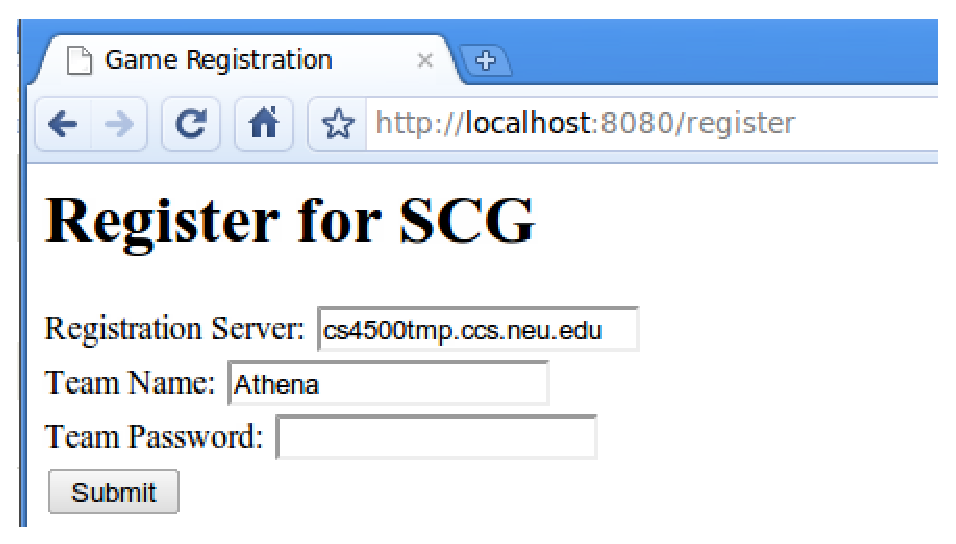
\includegraphics[width=100mm]{registration.eps}
\caption{Athena web based registration}
\label{fig:registration}
\end{figure}

By moving registration out of the command line arguments (as featured in the 
Basic Player), we eliminated a security risk. When an agent based on the Basic
Player runs, it publishes its team name and password on the machine process
tables. Some clever players took advantage of this, and ``registered'' all the
teams they had passwords for on a Tuesday competition without those teams
knowledge.

\textbf{Command line flags} were another crucial part of our agent. We designed
our code such that all magic numbers and constants were built as command line
flags. Anywhere we wanted to use such a value in the code base, we could call it
from a FLAGS global variable. Take our solver command like argument as an
example. Athena could be run with the solver flag,
\verb=./athena.py --solver c=, and then that value could be accessed anywhere
in our agent source as follows, \verb=print FLAGS.solver=, which yields ``c''.
This type of flexibility protects programmers from needing to pipe command line
processing from main methods all throughout their code. Along with the ease of
access, our flags library~\cite{gflags:website}, automatically generates
command line documentation for all the flags defined. This removes yet another
tedious development step.

\subsection{Competitive / Cooperative Nature}
% The game is competitive / cooperative.
% How did you react to the competitive nature of the game?

The competitive nature was a huge driving factor in getting us to write
the actual code. It was not, however, a factor in producing {\em good}
code. Some of the source code produced for competitions was in fact, awful. The
first competition that allowed multiple relation numbers, for example, Athena's
source code did not utilize all the relation numbers and only examined the
first for break-even calculation.

There was not much cooperation. Will's competition runner and Brent's
history viewer are nice tools, but they ultimately did not affect our
agent in a significant way.

\subsection{The need to do all steps well}
% Writing winning agents takes a lot of skill: at the conceptual,
% design and implementation level.
% If the conceptual understanding is perfect, but there is a flaw 
% in the design or implementation, your agent probably won't win. 
% How did you react to the need to do all steps well.

Writing the parser and creating the infrastructure (the straight-forward
parts that everyone can do) had virtually nothing to do with winning. All
the components that actually mattered were strenuous exercises in algorithm
design.

\subsection{Diversity}
% The success of such a class depends on having a community
% of students with different skills: Some like a more
% tactical approach, others strive for a strategic solution.
% Some are good programmers and others are not but they have other skills.
% Some like to use new tools and others only well tested tools.
% 
% How did you react to the diversity that was all focused through the game.

As the minority group, we did not encounter real diversity.

\subsection{Grades}
% How did you react to using the competition results as part of your grade?

We would not have minded so much if the code for the administrator was not
the specification.

\subsection{Feedback}
% Did the feedback you received through the competitions help
% you find bugs in your software?
Overall, competitions provided little feedback to us as software developers.
Because for the majority of the semester we were doing quite well, there was
little incentive to look over the rather convoluted game play logs to
determine where we were doing well, and where we needed to improve. Most of the
feedback garnered by our agent took the form of local competitions using the
runner tool. New features or other improvements were tested with the most
recently available administrator and other teams agent software. If we
continued to do well after a few sample group and tournament games, we
considered the new feature or improvement a success, and went for it in the
next competition.

This type of feedback model is ultimately flawed -- it relied on our team
believing that other teams would not improve enough game to game to exceeded
the level of improvement in our agent. 

\subsection{Observe, Design, Implement, Test}
% The other agents posed problems to you. Did the cycle:
% Observe history - Identify issues - Plan an approach - 
% Design your code - Implement - Test
% that you were exposed to after every competition help 
% you improve your problem solving skills?
There were no data mining efforts that made into the code base. Everything
was designed, implemented, then tested. Most of the design-implement-test cycle
was completed independent of external factors like game performance. We usually
had a feature list of things we wanted to implement, and weekly would try and
tackle at least one of them. This pace happened to coincide with features
needed to stay on the upper edge, but this was not a cause and effect
relationship.

We did look at the history files of the games where we lost, but we didn't
let it sway how we implemented the code. Game history files were too much of
a burden to study regularly. They contain a great deal of information, while
only a small percentage of the total is useful to individual teams.

\subsection{Problems created by your peers}
% Many software design and implementation problems you had to solve during the course
% were caused by your peers. I only made sure through the game design
% that they could pose reasonable problems to you.
% Did the fact that you solved problems created by your peers
% motivate you?
We were not motivated directly by our peers. Other teams merely provided a test
data set for the soundness of our algorithms. In general, it seemed that the
best approach to this problem was to design a solution that worked in the
general case. Special case ``hacks'' were seldom made, as they tended to be
extremely fragile. 

\subsection{SCG skills}
% The SCG game was designed so that it is sound, i.e.,
% the game score reflects **only** the agent's skill level in:

\subsubsection{Solving problems}

This skill is seldom tested, since the game itself is not a benchmark on
the solver alone. There have been games were no problems were solved. There
have been games were only one agent solved. So, even logically, the game is
not a reflection on the solver.

\subsubsection{Providing hard problems}

Same thing for this skill. There can be an instance of a game were nothing
is ever provided (only offers and re-offers).

\subsubsection{Introspective skills}

% Argue for or against soundness of the SCG game.

\subsection{SCG game}
% 2.9
% The game was designed so that it has the following 3 properties:

\subsubsection{An agent can't force other agents to consistently lose}
\subsubsection{An agent can't force other agents to consistently draw}
\subsubsection{An agent can't force other agents to consistently win}

% Argue for or against those 3 properties of the SCG game.
% 
% The entire document should not be longer than 7 pages. 
%
\bibliography{finalproject}{}
\bibliographystyle{IEEEtran}
\end{document}
